\documentclass{article}

% spanish-inputenc
% longtable for reportable
% echo in chunk
% results in latex
% par(mfrow=c(filas,columnas))
% statgazer and report table packages

\usepackage[utf8]{inputenc}
\usepackage{longtable}

\usepackage{Sweave}
\begin{document}
\Sconcordance{concordance:paperVersion_1.tex:paperVersion_1.Rnw:%
1 12 1 1 0 18 1 1 12 3 1 1 10 42 0 1 2 3 1 1 39 1 2 2 1 1 5 15 0 1 2 5 %
1 1 5 12 0 1 2 4 1 1 9 14 0 1 2 4 1 1 5 1 1 1 2 34 0 1 2 18 1}


LOS INDICES DEL MUNDO


Por: Estrella Delcurso


Introducción

Aqui les presento mi investigacion sobre diversos indices sociales en el mundo. Los indices los conseguí de wikipedia, espero que les gusten mucho.


Exploración Univariada

En esta sección exploro cada índice.




Este es el comportamiento de las variables a estudiar. Veamos su tabla de frecuencias:

% latex table generated in R 3.4.1 by xtable 1.8-2 package
% Tue May 29 09:25:20 2018
\begingroup\footnotesize
\begin{longtable}{llrrr}
\caption{Tablas de Frecuencia de la variables en estudio} \\ 
 \textbf{Variable} & \textbf{Levels} & $\mathbf{n}$ & $\mathbf{\%}$ & $\mathbf{\sum \%}$ \\ 
  \hline \hline
WorldFreedom & 1 & 55 & 26.7 & 26.7 \\ 
   & 3 & 62 & 30.1 & 56.8 \\ 
   & 5 & 89 & 43.2 & 100.0 \\ 
   \hline
 & all & 206 & 100.0 &  \\ 
   \hline
\hline
EconomicFreedom & 1 & 21 & 10.1 & 10.1 \\ 
   & 2 & 78 & 37.7 & 47.8 \\ 
   & 3 & 74 & 35.8 & 83.6 \\ 
   & 4 & 28 & 13.5 & 97.1 \\ 
   & 5 & 6 & 2.9 & 100.0 \\ 
   \hline
 & all & 207 & 100.0 &  \\ 
   \hline
\hline
PressFreedom & 1 & 22 & 10.7 & 10.7 \\ 
   & 2 & 53 & 25.7 & 36.4 \\ 
   & 3 & 66 & 32.0 & 68.5 \\ 
   & 4 & 48 & 23.3 & 91.8 \\ 
   & 5 & 17 & 8.2 & 100.0 \\ 
   \hline
 & all & 206 & 100.0 &  \\ 
   \hline
\hline
Democracy & 1 & 60 & 29.1 & 29.1 \\ 
   & 2 & 45 & 21.8 & 51.0 \\ 
   & 4 & 82 & 39.8 & 90.8 \\ 
   & 5 & 19 & 9.2 & 100.0 \\ 
   \hline
 & all & 206 & 100.0 &  \\ 
   \hline
\hline
\hline
\label{}
\end{longtable}
\endgroup

Una vista gráfica a lo anterior la tenemos a continuación:

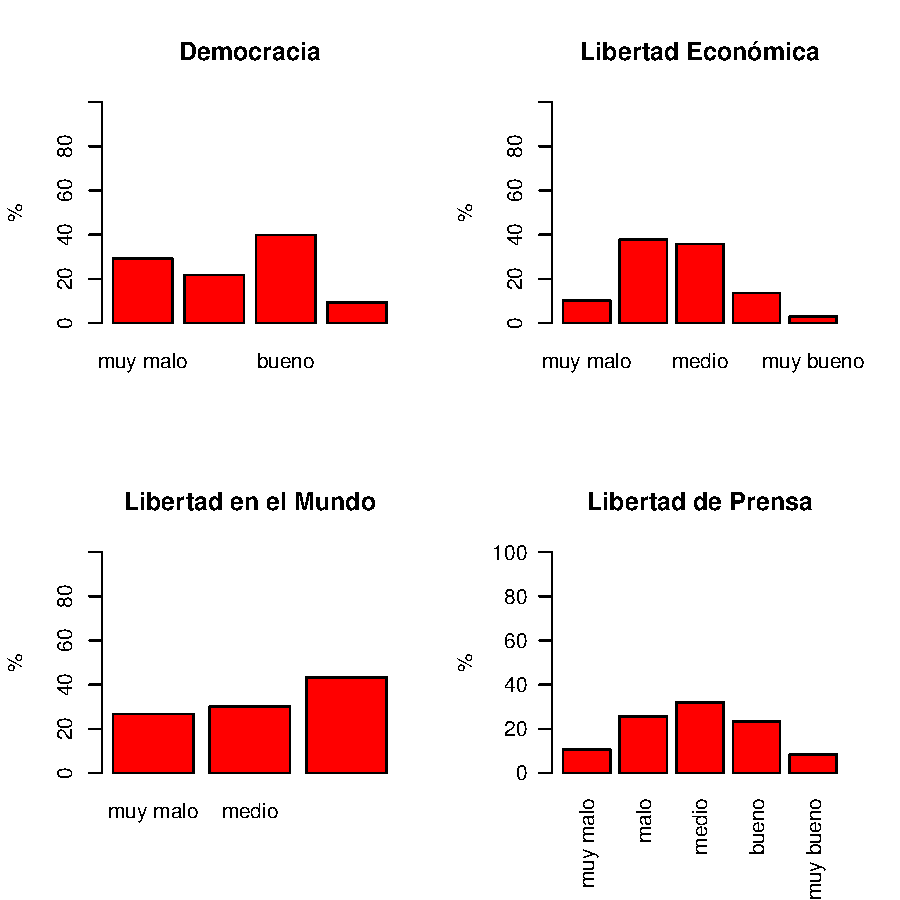
\includegraphics{paperVersion_1-demoTable}


Podemos mostrar los estadísticos de cada variable:
% Table created by stargazer v.5.2 by Marek Hlavac, Harvard University. E-mail: hlavac at fas.harvard.edu
% Date and time: Tue, May 29, 2018 - 09:25:20
\begin{table}[!htbp] \centering 
  \caption{Medidas estadísticas} 
  \label{} 
\begin{tabular}{@{\extracolsep{5pt}}lcc} 
\\[-1.8ex]\hline 
\hline \\[-1.8ex] 
Statistic & \multicolumn{1}{c}{N} & \multicolumn{1}{c}{Median} \\ 
\hline \\[-1.8ex] 
WorldFreedom & 206 & 3 \\ 
EconomicFreedom & 207 & 3 \\ 
PressFreedom & 206 & 3 \\ 
Democracy & 206 & 2 \\ 
\hline \\[-1.8ex] 
\end{tabular} 
\end{table} 

Exploración Bivariada

En este trabajo estamos interesados en el impacto de los otros indices en el nivel de Democracia. Veamos las relaciones bivariadas que tiene esta variable con todas las demás:

% Table created by stargazer v.5.2 by Marek Hlavac, Harvard University. E-mail: hlavac at fas.harvard.edu
% Date and time: Tue, May 29, 2018 - 09:25:24
\begin{table}[!htbp] \centering 
  \caption{Correlación de Democracia con las demás variables} 
  \label{} 
\begin{tabular}{@{\extracolsep{5pt}} ccc} 
\\[-1.8ex]\hline 
\hline \\[-1.8ex] 
WorldFreedom & EconomicFreedom & PressFreedom \\ 
\hline \\[-1.8ex] 
$0.896$ & $0.587$ & $0.771$ \\ 
\hline \\[-1.8ex] 
\end{tabular} 
\end{table} 

Veamos la correlación entre las variables independientes:


% Table created by stargazer v.5.2 by Marek Hlavac, Harvard University. E-mail: hlavac at fas.harvard.edu
% Date and time: Tue, May 29, 2018 - 09:25:24
\begin{table}[!htbp] \centering 
  \caption{Correlación entre variables independientes} 
  \label{} 
\begin{tabular}{@{\extracolsep{5pt}} cccc} 
\\[-1.8ex]\hline 
\hline \\[-1.8ex] 
 & WorldFreedom & EconomicFreedom & PressFreedom \\ 
\hline \\[-1.8ex] 
WorldFreedom & 1 &  &  \\ 
EconomicFreedom & 0.49 & 1 &  \\ 
PressFreedom & 0.83 & 0.53 & 1 \\ 
\hline \\[-1.8ex] 
\end{tabular} 
\end{table} 



Finalmente, vemos los modelos propuestos. Primero sin la libertad mundial como independiente, y luego con está :


% Table created by stargazer v.5.2 by Marek Hlavac, Harvard University. E-mail: hlavac at fas.harvard.edu
% Date and time: Tue, May 29, 2018 - 09:25:24
\begin{table}[!htbp] \centering 
  \caption{Modelos de Regresión} 
  \label{} 
\begin{tabular}{@{\extracolsep{5pt}}lcc} 
\\[-1.8ex]\hline 
\hline \\[-1.8ex] 
 & \multicolumn{2}{c}{\textit{Dependent variable:}} \\ 
\cline{2-3} 
\\[-1.8ex] & \multicolumn{2}{c}{Democracy} \\ 
\\[-1.8ex] & (1) & (2)\\ 
\hline \\[-1.8ex] 
 WorldFreedom &  & 0.704$^{***}$ \\ 
  &  & (0.046) \\ 
  & & \\ 
 EconomicFreedom & 0.377$^{***}$ & 0.291$^{***}$ \\ 
  & (0.077) & (0.053) \\ 
  & & \\ 
 PressFreedom & 0.833$^{***}$ & 0.012 \\ 
  & (0.065) & (0.070) \\ 
  & & \\ 
 Constant & $-$0.642$^{***}$ & $-$0.354$^{**}$ \\ 
  & (0.199) & (0.138) \\ 
  & & \\ 
\hline \\[-1.8ex] 
Observations & 206 & 206 \\ 
R$^{2}$ & 0.637 & 0.830 \\ 
Adjusted R$^{2}$ & 0.634 & 0.828 \\ 
Residual Std. Error & 0.880 (df = 203) & 0.603 (df = 202) \\ 
F Statistic & 178.197$^{***}$ (df = 2; 203) & 329.420$^{***}$ (df = 3; 202) \\ 
\hline 
\hline \\[-1.8ex] 
\textit{Note:}  & \multicolumn{2}{r}{$^{*}$p$<$0.1; $^{**}$p$<$0.05; $^{***}$p$<$0.01} \\ 
\end{tabular} 
\end{table} 

















\end{document}
